%---------------------------------------------------------------------------------------------------
% Francisco Gimenez
% April, 2015
% PhD Dissertation Proposal
% Stanford University, Program in Biomedical Informatics
%
%---------------------------------------------------------------------------------------------------

%---------------------------------------------------------------------------------------------------
% Packages

\documentclass[12pt,twoside]{report}		% double-sided for binding. font size: 10, 11, or 12 pt.
\usepackage{config/suthesis-2e-poznik}             % Stanford Dissertation .sty file, with my edits
\usepackage{amsmath}						% mathematical formulas
\usepackage{amssymb}						% mathematical symbols
\usepackage{graphicx}						% \includegraphics for eps and pdf graphics
\usepackage{cite}							% to clean up citations in the main text
\usepackage[labelfont=bf,labelsep=period]{caption}	% bold figure number in caption
\usepackage{subcaption}						% for subfigures
\usepackage{color}							% to color text: {\color{red} text}
\usepackage[usenames,dvipsnames]{xcolor}	% more flexibility for colors
\usepackage{amsfonts}						% \mathcal, \mathbb, \mathscr, etc
\usepackage{amsthm}							% \newtheorem{name}{Printed output}
\usepackage{amscd}							% rectangular diagrams
\usepackage{verbatim}						% reproduce every char w/in \begin{verbatim} ... 
\usepackage{epstopdf}						% convert eps to pdf
\usepackage[backref]{hyperref}				% hyperlinks; backrefs in bibliography
\usepackage[nameinlink,noabbrev]{cleveref}  % capitalize at start of sentence
\usepackage{setspace}						% for line-spacing
\usepackage{fancyhdr}						% enables fine control over headers and footers
\usepackage[super]{nth}						% for super-scripting 1st, 2nd, etc.
\usepackage{courier}    					% sets \ttfamily to courier new
\usepackage{rotating}						% for rotating figures and captions
\usepackage{afterpage}						% for placement of rotated figures and captions
\usepackage{booktabs}						% to make book-quality tables
\usepackage{bm}								% enables boldface in math mode with \boldsymbol{}
\usepackage{multirow}						% enables spanning multiple rows in a table
\usepackage{fixltx2e}						% enables \textsubscript{}
\usepackage{float}							% enables H to force figure placement here
%\usepackage{macros}							% .sty file with all my macros

%---------------------------------------------------------------------------------------------------
% Electronic submission:
% * Set \onlinetrue: removes copyright and signature pages
% 
% Actual dissertation:
% * Comment out \proposaltrue
% 	a. removes "proposal" from title page
% 	b. includes acknowledgments
% * Comment out proposed work chapter and uncomment discussion chapter.

\proposaltrue								% affects title page, acknowledgements, final chapter
%\onlinetrue								% electronic submission: remove copyright and signature pages

%---------------------------------------------------------------------------------------------------
% Includeonlies. To compile a shorter list of .tex files.

%\includeonly{abstract,preface,chapter1-introduction}

%---------------------------------------------------------------------------------------------------
% Bibliography

% bibliography style
\bibliographystyle{unsrt}					% bibtex style. e.g., plain (sorted), unsrt, plos2009
%\makeatletter								% enables usage of @ in package modification
%\renewcommand{\@biblabel}[1]{\quad#1.}		% remove brackets from numbering in list of references
%\makeatother								% returns @ to normal usage
%\renewcommand*{\backref}[1]{[#1]}			% format back references in bibliography

%---------------------------------------------------------------------------------------------------
% Settings

% hyperlinks
\definecolor{linkCol}{RGB}{23,118,153}		% yields plos genetics color: 23,98,135
\hypersetup{
    colorlinks,								% colors text rather than surrounding it by a box
    linkcolor={linkCol},					% internal links
    citecolor={blue!50!black},				% citations: 50% blue, 50% black
    urlcolor={blue!80!black}				% web links and urls: 80% blue, 20% black
}

%---------------------------------------------------------------------------------------------------
% Title Data

\title{Fast Adaptive Structured Reporting to Improve Radiological Performance}
\author{Francisco J. Gimenez}
\programthesis
\dept{Biomedical Informatics}
\principaladviser{Daniel Rubin}
\firstreader{Ross Shachter}
\secondreader{Mark Musen}

%---------------------------------------------------------------------------------------------------
% Start Document

\begin{document}
\beforepreface						% title, copyright, and signature pages

%---------------------------------------------------------------------------------------------------
% Prefaces. Each must begin with: \prefacesection{myTitle}.

\prefacesection{Abstract}
Radiology is a powerful tool to detect and diagnose abnormalities by allowing doctors to visually inspect internal pathology that could not otherwise be seen. However, assessing radiological images is limited by variations among practitioners, including deficiencies in their reporting of these imaging examinations as well as in their interpretations. Three main sources of these variations in interpretation are incorrectness of observations in the images, incompleteness of the radiological observations reported to characterize the abnormalities, and inconsistency of these observations with respect to the radiologists' overall impression. We hypothesize that the quantification and enforcement of correctness, completeness, and consistency of radiological observations will improve the diagnostic accuracy and reduce variability of interpretation. To test this hypothesis, we propose a decision support system that provides feedback to radiologists during the reporting of their radiological observations. We will develop this system by creating novel statistical models to link radiological observations, computational imaging features, and disease to recognize incorrectness, incompleteness and inconsistency in reporting. We will then harness these models to create a quantifiable metric of observation quality. We propose a research plan with the following specific aims: (1) To characterize breast lesions seen in mammography images by capturing computationally-derived (``quantitative'') imaging features and radiologist-derived observational (``semantic'') features, (2) develop metrics to measure incorrectness, incompleteness, and inconsistency, and (3) develop a decision-support system to improve these metrics. We will test this system in mammography, and show how it can be extended to other imaging domains and possibly to other medical domains where diagnostic reasoning is documented in dictated reports.


\prefacesection{Preface}

Preface goes here
\ifproposal 						% exclude acknowledgements from proposal
\else \prefacesection{Acknowledgements}
If this dissertation was 100 times longer, I still would not be able to hand out a souvenir page to all the amazing people in my life who have helped me along the way. That being said, I want to make explicit the gratitude I show to several of my friends and mentors.

To my advisor Daniel Rubin, you have been exactly everything I needed to do this work. You gave me enough freedom to grow as a research on my own while still providing enough guidance such that I didn't get lost in the purgatory of aimless projects. Whatever skills and success I have as a scientist are due in large part to how you showed me how to think.

To my committee members Ross Shachter, Mark Musen, and Curt Langlotz, thank you for the extremely entertaining and enlightening conversations. Ross, you challenged me like no other and always caught my mistakes in reasoning. It has made your approval so much more worthwhile. Mark, I would often find myself floating around MSOB looking to talk shop, and you would always indulge me if you had the time. It was always worth stopping by to talk about research and life in general. Curt, I am pretty annoyed you took so long to come to Stanford given how helpful you have been to me in the past year and half. I don't think I could ever approach being as smart as you, but I'll sure as hell try.

To BMI faculty and staff, you made the program feel more like a family than graduate school. Thank you MaryJeanne Oliva, Nancy Lennartson, John DiMario, Russ Altman, Nigam Shah, Dennis Wall, and David Paik. Stanford seemed like an intimidated place to go to graduate school until I met you all and felt welcomed.

To the Bankiewicz lab, especially Krys, John, Piotr, Mishek, and old Francisco. You taught me that research was my calling and were one of the biggest influences on my future. Thanks for taking a chance on my 20 year old self however annoying I may have been.

To my outstanding high school teachers, you taught me to love learning. Mr. Tastor, Mr. Fisher, Mrs. Kars, Mr. Westberg, whatever seed you planted in me remained today (for better or for worse).

To my BMI colleagues, you have been the best peers, friends, therapists, and guardians. Brian you were a great roommate, friend, and surfing buddy and are likely one of the funniest people I know. Jonathan, I thought you were extremely weird when I first met you, and I haven't really changed my mind about that, but you have come to be such a wonderful partner in crime. Beth, it has been a pleasure learning about life with you on our frequent coffees and beers. Katie, you always keep me on a tight leash, but you are easily the most dependable friend anybody could have. Diego, thanks for being my video game sherpa and carrying so hard. Pablo, we formed a Latino czar dream team that will never be beaten. Moskowitz, your love of food and sense of humor pretty much means I will always make time to hang out with you. Dpoz, you are easily one of the most dedicated and honest people I know, and I will always secretly try emulate that. Sarah, thank you so much for being an acceptor of all things weird; I wish you stayed around us a little longer. There are likely a lot of you I missed, take this section as an opportunity to call me out on it and I'll buy you a beer.

To Mom, Dad, Alfredo, Ari, and Lisa, you are the best family I could have. I know no better times than spending time with you all, and hard times have been a breeze knowing you were there for me. I am forever indebted and hope I give you a fraction of the support, joy, comfort, and love you have given me.

Finally, I would like to thank my funding sources the National Library of Medicine Training Grant (LM007033) and the National Institutes of Health for my Ruth L. Kirchstein National Research Service Award Fellowship (1F31CA171789-01A1 ).  \fi	

%---------------------------------------------------------------------------------------------------
% Post-Preface Front Matter

{ \hypersetup{hidelinks}			% keep TOC black
  \contentstablesfigures }			% tables of contents, tables, and figures
\startmaindoc						% start main body: \cleardoublepage, arabic page 1, headings

%---------------------------------------------------------------------------------------------------
% Chapters. Each must begin with: \chapter{myChapterTitle}.

\chapter{Introduction}
Radiology is a powerful tool to detect and diagnose abnormalities by allowing doctors to visually inspect internal pathology that could not otherwise be seen. Though it is an indispensable part of the diagnostic workup, the practice of radiology is still fraught with error due to the inherently subjective nature of the task; the doctor must still visually scan, detect, and interpret the findings in the image to deliver an impression. An unfortunate consequence of such a system is substantial variability in practice and performance. This dissertation aims to tackle these shortcomings. To do so, I propose a novel computational decision-support paradigm aimed at improving the quality and content of the radiological \emph{report} rather than the traditional approaches aimed at directly improving the diagnosis. I develop informatics methods within this paradigm to detect and reduce error in reports, and show how these methods have the potential to improve overall diagnostic performance. This chapter provides an overview of the dissertation. I begin by providing a brief background of radiological error, decision-support systems, and reporting. I then give a high-level description of my proposed decision-support model, methods, and key results. Finally, I delineate my contributions to the field and provide a guide to the reader for the remainder of the document.

\section{Radiology, variability, and errors}
Radiology is an essential part of modern clinical medicine, constituting 10.6\% of health care spending and is virtually ubiquitous in every part of health care \cite{Dodoo:tg}. The field has traditionally been at the forefront of medical technology by virtue of its foundations and reliance upon sophisticated technological achievements. Digital radiology and picture archiving and communications systems led to an early, widespread adoption of electronic records with respect to imaging \cite{Strickland:2000cv,Bryan:1999kn}. But, despite the early adoption of computational systems to manage data, the actual practice of radiology remains a relatively unchanged. An unfortunate consequence of such a system is substantial variability in practice and performance \cite{Fitzgerald:2001hn}. \citeA{Robinson:1997uq} went so far as to state that ``errors and variations in interpretation now represent the weakest aspect of clinical imaging'' and declared such issues as ``Radiology's Achilles' heel''. This is not to say that radiologists are the only doctors faced with these issues, as the now infamous Institute of Medicine report \emph{To Err is Human: Building a Safer Health System} revealed a striking amount of poor patient outcomes are a result of medical error \cite{Anonymous:2000va}. A prominent recommendation from this study is the use of automation and computation to improve upon standard of care via decision support systems.

\section{Radiological decision-support}
Decision support systems are tools that incorporate medical information to provide meaningful input to medical practitioners. The main source of medical information in radiology is confined to patient history drawn from the electronic medical record, the patient images, and the reports generated by the radiologists. As a result, it is a ripe domain for decision support tools to assist in organizing, analyzing, and synthesizing these data sources. 

Radiological data mining allows clinicians to query similar cases to the ones they are evaluating \cite{Shin:2015wl,Bozkurt:2014jw,Depeursinge:2012ce,Korenblum:2011gx,Akgul:2011ey,Nassif:2009du}. Computer-aided detection (CADe) systems assist in identifying abnormalities in images across a variety of radiological domains such as mammography, colonoscopy, lung screening, and liver diagnosis \cite{Cheng:2003ig,Castellino:2005ke,Meeuwis:2010bv,Oliver:2010fm,Fenton:2011fw,Fenton:2012kz,Jamieson:2012hz,Gallas:2012eg,Giger:2013jb}. Computer-aided diagnosis (CADx) systems assist in interpretation of abnormalities found in the image \cite{Jiang:1999fj,ElizabethS:2005gc,Gallas:2012eg,Bright:2012ga,Giger:2013jb,Depeursinge:2010jl,Fujita:2008it,Eadie:2011cv,Rubin:2005jg,Garg:2005cb,Elter:2009fv,Jamieson:2010vl,Jamieson:2010tt,Cheng:2003ig,Jiang:2001fy} as well as interpretation of the content within the radiology report \cite{Burnside:2000wl,ElizabethS:2005gc,Burnside:2009br,Rubin:2005jg}.

Despite significant technological achievements, adoption of these systems in radiology is limited. In particular, the only commercially deployed radiological decision support systems are computer-aided detection (CADe). The main reasons for this inability to affect practice is that these systems often interrupt clinical  work-flow, give assessments rather than recommendations, and fail to provide decision-support during decision-making \cite{Kawamoto:2005gn,Morgan:2011ct}. These shortcomings are not unique to radiological decision support; they exhibit the same symptoms of decision support systems in other clinical domains that did not see commercial adoption. In general, they still follow the the so-called \emph{Greek Oracle} model of decision support \cite{Miller:1990wg,Miller:1994cx}. Such systems fail when deployed in practice since they are based on the implicit assumption that computers can perform the duties of doctors better than doctors themselves. Charles Friedman goes so far as to declare that the \emph{Fundamental Theorem of Biomedical Informatics} is that decision support should ``augment human reasoning'' beyond the capabilities of an unaided practitioner \cite{Friedman:2009dx}. Thus, it is crucial to develop radiological decision support tools that fit into the work-flow and augment their reasoning. A perfect window to provide this is during radiological reporting.

\section{Radiology reporting}
The radiology report conveys the radiologist's findings, interpretation of these findings, and suggested patient management. It is also the primary form of communication of this information to referring clinicians or patients \cite{Sistrom:2005cx}. Given that communication breakdowns constitute 80\% of medical malpractice lawsuits \cite{Levinson:1994ko}, and radiological reports are legally admissible court documents \cite{Oppenheim:2012tq}, considerable effort has been made to measure and improve upon report quality \cite{Langlotz:2015vq}. These studies have identified key tenets of report quality: correctness of findings, completeness of the description of significant clinical findings, consistency of report language and findings, and timeliness of the report's completion \cite{Johnson:2004kh, HaraldO:2004hi, Reiner:2006fa}. 

Several projects aim to improve the quality of radiology reports. Standardization of mammography reporting via the Breast Imaging Reporting and Data System (BI-RADS) has led to uniform reporting language and assessment guidelines \cite{Liberman:ws,Langlotz:2009fn,Burnside:2009ki}. RadLex is an effort to extend standardization of terminology by defining a lexicon of all radiological concepts \cite{Langlotz:2006jn}. In addition to terminology, there is a strong push to create \emph{structured reports} that further standardize report format and organization \cite{Langlotz:2009dd,Reiner:2009ib}. Structured reports not only can improve communication, but they allow for computability of the report information beyond the constraints of free-text documents. Unfortunately, structured reporting is not without its drawbacks. It requires new software to implement into the clinical work flow which is costly in terms of implementation and training. More importantly, structured report creation is time-intensive and imposes distractions in the traditional radiological work flow, directly interfering with timeliness \cite{Weiss:2008er}. Despite these shortcomings, structured reporting is widely seen as the future of radiological reporting \cite{Langlotz:2015vq}.

Both standardized terminology and structured reports are solid steps to improving upon the reporting process, but they do not directly analyze the radiological concepts being communicated. Borrowing from the \emph{meaning triangle}, the tools described encode radiological objects with standard expressions, but they do not encode their sense or concept \cite{Mead:2006wm}. Such work would need to perform higher order analysis of the information in the report including, but not limited to, analyzing if the contents in the reports is correct, complete, or even consistent with diagnosis. In this sense, decision support systems provide the missing piece for this analysis.

\section{Providing decision support during reporting time}

My hypothesis is that delivering decision support during reporting time to improve completeness and correctness of reports will improve consistency, and therefore, diagnostic performance. To this end, I seek to answer the following questions:

\paragraph{How can we improve the quality of radiological report?}

Though I have described methods to improve the terminology and format of the report, there is much to be done to improve upon the \emph{content} of the report. What can we do to improve upon this information? How can we actually implement such solutions?

\paragraph{Does improving the report improve diagnostic performance?}

There are no studies showing that improving the content of the radiological report can actually improve the diagnostic performance of the physician. If we implement new methods to improve the report, will they have any effect on the radiologist's outcome? Otherwise, are we needlessly burdening radiologists with technology to fix reporting for its own sake?

\subsection{Specific Aims}

\begin{enumerate}
	\item Develop methods to assess completeness and correctness of radiology reports
	\item Evaluate these methods in two important radiological domains (mammography and liver CT)
	\item Use completeness and correctness metrics to provide feedback to improve consistency and diagnostic performance
\end{enumerate}

\subsection{Methodology}

\begin{figure}[h]
	\centering
	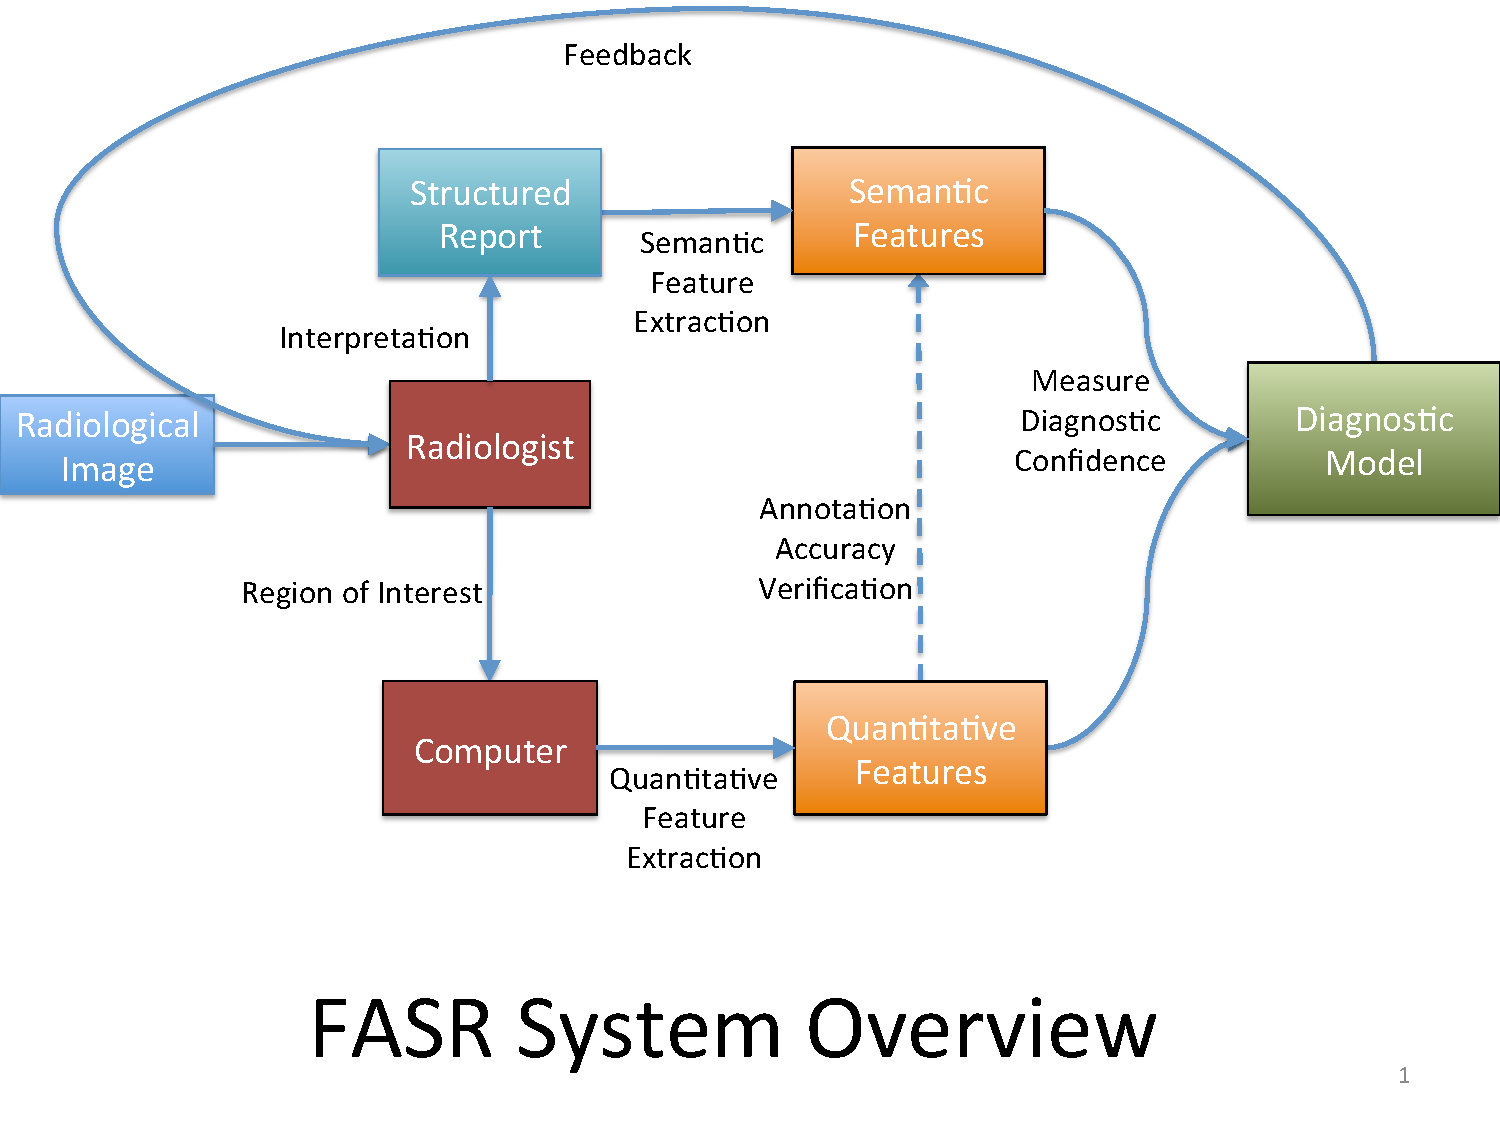
\includegraphics[width=1\linewidth]{fasr_diagram.pdf}
	\caption{Overview of the Fast Adaptive Structured Reporting (FASR) system}
	\label{fig:fasr_diagram}
\end{figure}

To tackle this challenge and to enable translation of decision-support system into clinical practice to benefit patient care, I propose a real-time decision-support system that provides feedback to radiologists as they generate their reports called Fast Adaptive Structured Reporting (FASR). This system will create evaluate and improve upon the content of a structured radiological report. This differs from traditional approaches to decision-support system because our system will improve upon reporting, and by our hypothesis, implicitly improve upon practice. By ensuring that the relevant observations are correctly, completely, and consistently described in mammography reports, our decision-support system will reduce variability in practice, improving practitioner decision making and lead to better patient care.

\subsection{Key Results}


\section{Summary of contributions}
This work demonstrates contributions to the our understanding of reporting in radiology as well as performance of decision-support systems for diagnostics.

\subsection{Radiology contributions}
\subsubsection{Automatic annotation and verification of descriptors in liver CT scans}
\subsubsection{Correlated incomplete reports with diagnostic error}

\subsection{Informatics Contributions}
\subsubsection{General purpose semantic classification of images}
\subsubsection{Monte-Carlo computation of same-decision probability}
\subsubsection{Framework for delivering and evaluating feedback in decision-support systems}


\section{Guide for the reader}

\chapter{Background}

%\section{Radiology Reporting}

\section{Liver Imaging}
\subimport{}{liver_background}

\section{Mammography}
\subimport{}{mammo_background}



%\section{Probabilistic Graphical Models}
\chapter{FASR: Fast Adaptive Structured Reporting}

%%%%%%%%%%%%%%%%%%%%%%%%%%%%%%%%%%%%%%%%%%%%%%%%%%%%%%%%%%%%%%%%%%%%%%%%%%%%%%%
% FASR DESCRIPTION
%%%%%%%%%%%%%%%%%%%%%%%%%%%%%%%%%%%%%%%%%%%%%%%%%%%%%%%%%%%%%%%%%%%%%%%%%%%%%%%

\section{Annotation Verification}
\subsection{Human-Derived Imaging Features}
\subimport{}{liver_method}
\subsection{Deep Learning Features}

\section{Completeness Calculation}
\subimport{}{completeness_method}

\section{Decision Support Feedback}


\chapter{Results}

\section{Annotation Verification}
\subimport{}{liver_results}

\section{Completeness Calculation}
\subimport{}{completeness_results}

\section{Decision Support Feedback}


%---------------------------------------------------------------------------------------------------
% Appendices. Each must begin with: \chapter{myAppendixTitle}.

%\appendix
%\include{appendixFN}

%---------------------------------------------------------------------------------------------------
% Bibliography and dismount.

\bibliography{bib/bibtex_lib_04-13-2015.bib}		% full path to .bib (bibtex file)
\end{document}
